Volem construir un petit cobert de fusta de $6\ \text{m}^3$ de volum, en forma de prisma rectangular, adossat a la
paret lateral d'una casa, per a guardar-hi llenya. Només cal construir, per tant, el sostre i tres parets (la
paret del fons del cobert és la de la casa a la qual està adossat). A més, volem que el cobert mesuri el triple
d'amplària que de fondària. Cada metre quadrat de paret té un cost de construcció de 30 € i el sostre costa 50 €
per metre quadrat. Un cop construït el cobert, afegir-hi una porta té un cost fix de 35 €.
\begin{center}
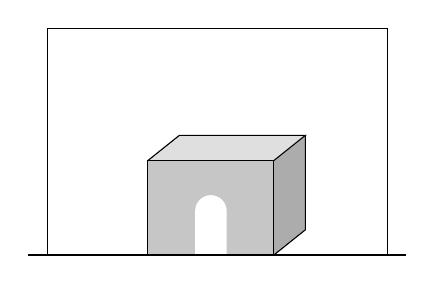
\begin{tikzpicture}[scale=0.8]
  \draw (0,0) -- (0,3.6) -- (5.4,3.6) -- (5.4,0);
  \fill[gray!45] (1.6,0) rectangle (3.6,1.5);
  \fill[gray!25] (1.6,1.5) -- (2.1,1.9) -- (4.1,1.9) -- (3.6,1.5) -- cycle;
  \fill[gray!65] (3.6,0) -- (4.1,0.4) -- (4.1,1.9) -- (3.6,1.5) -- cycle;
  \draw (1.6,0) rectangle (3.6,1.5);
  \draw (1.6,1.5) -- (2.1,1.9) -- (4.1,1.9) -- (3.6,1.5);
  \draw (3.6,0) -- (4.1,0.4) -- (4.1,1.9);
  \fill[white] (2.35,0) -- (2.35,0.7) arc[start angle=180,end angle=0,radius=0.25] -- (2.85,0) -- cycle;
  \draw (-0.3,0) -- (5.7,0);
\end{tikzpicture}
\end{center}

\begin{apartats}

\apartat{1,25}
Comproveu que el cost de construcció del cobert ve donat per la funció $C(x)=\dfrac{300}{x}+150x^2+35$, on $x$ és
la fondària del cobert en metres.

\begin{solucio}
Com s'indica a l'enunciat, denotem per $x$ la fondària del cobert, i per $h$, l'alçada; l'amplada serà $3x$. El
volum del cobert ha de ser de $6\ \text{m}^3$, és a dir, $3x\cdot x\cdot h=6$ i, per tant, $h=\frac{2}{x^2}$. El
cost de construcció és donat per
\[
C(x)=30\cdot(3xh+xh+xh)+50\cdot3x^2+35=150xh+150x^2+35=150x\cdot\frac{2}{x^2}+150x^2+35=\frac{300}{x}+150x^2+35 .
\]

\textit{Pauta oficial:} 0,25 pel plantejament correcte de les variables (amplada, fondària i alçada), 0,5 per
expressar la lligadura que representa el volum fixat, i 0,5 per l'expressió final del cost. També poden plantejar
que l'amplada és $x$ i la fondària $\frac x3$: els càlculs seran diferents, però doneu els punts corresponents de
cada part sempre que estigui ben feta i ben argumentada.
\end{solucio}

\apartat{1,25}
Calculeu quines han de ser les dimensions del cobert per tal que el cost de construcció sigui mínim, i
justifiqueu la resposta. Quin és aquest cost?

\begin{solucio}
Per minimitzar la funció $C(x)$, calculem-ne la derivada: $C'(x)=-\dfrac{300}{x^2}+300x$. Si resolem l'equació
$C'(x)=0$, obtenim $\frac{300}{x^2}=300x$ o, equivalentment, $x^3=1$, que té com a única solució real $x=1$.
Com que $C''(x)=\frac{600}{x^3}+300$ i $C''(1)>0$, comprovem fàcilment que es tracta d'un mínim de la funció.
Així doncs, les dimensions del cobert han de ser $x=1$ metre de fondària, $3x=3$ metres d'amplada i
$h=\frac{2}{1^2}=2$ metres d'alçada. Per a aquestes dimensions, el cost de construcció és de
$C(1)=\frac{300}{1}+150\cdot1^2+35=485$ euros.

\textit{Pauta oficial:} 0,25 per la derivada, 0,25 per aïllar correctament, 0,25 per justificar que es tracta
d'un mínim, 0,25 per les tres dimensions demanades i 0,25 pel càlcul del cost total. La justificació del mínim
també es pot fer sense la derivada segona, analitzant el signe de la derivada primera: compteu-ho bé si ho fan
així, sempre que estigui ben argumentat.
\end{solucio}

\end{apartats}
